% Model - med figur
% Algorithm - som figur
% Animationer
% Demo af sumo

\section{Solution}
\subsection{Model}
\begin{frame}{Model}
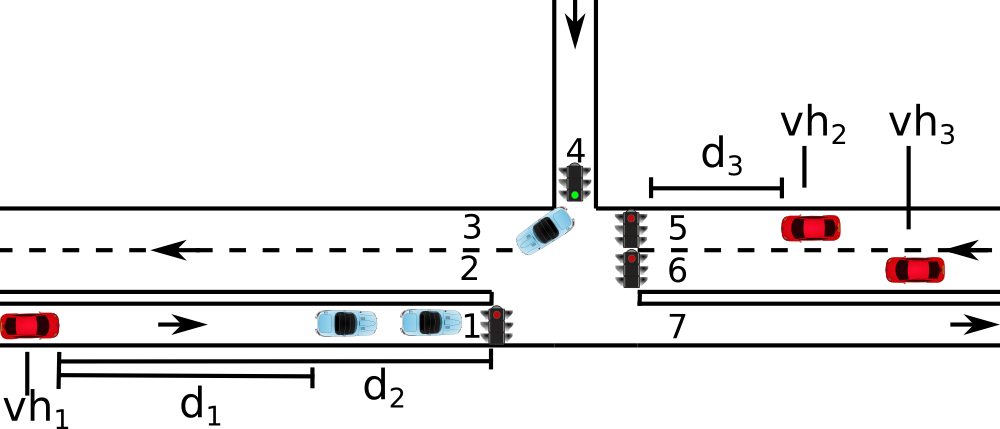
\includegraphics[width=1\textwidth]{images/introNetwork.png}
\end{frame}

\begin{frame}{Space Model}
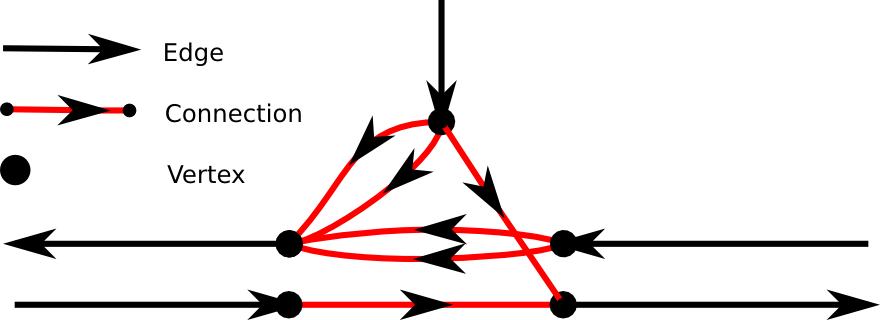
\includegraphics[width=1\textwidth]{images/ConnectionNetwork.png}
\end{frame}

\subsection{Algorithm}
\begin{frame}{Algorithm}
\begin{itemize}
\item In a junction
\item Calculate distance
\item Phase conversion
\item Calculate velocity
\end{itemize}
\end{frame}
\begin{frame}{In Junction}
\begin{center}
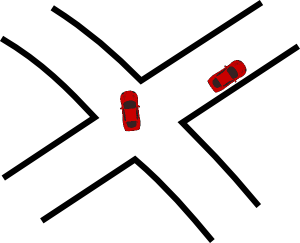
\includegraphics[width=0.8\textwidth]{images/algjuction.png}
\end{center}
\end{frame}

\begin{frame}{Calculate Distance}
\begin{center}
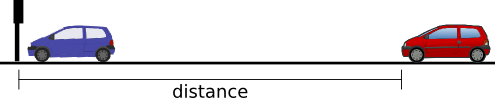
\includegraphics[width=1\textwidth]{images/algdistance.png}
\end{center}
\end{frame}

\begin{frame}{Phase Conversion}
\begin{columns}
	\begin{column}{0.3\textwidth}
	\begin{center}
	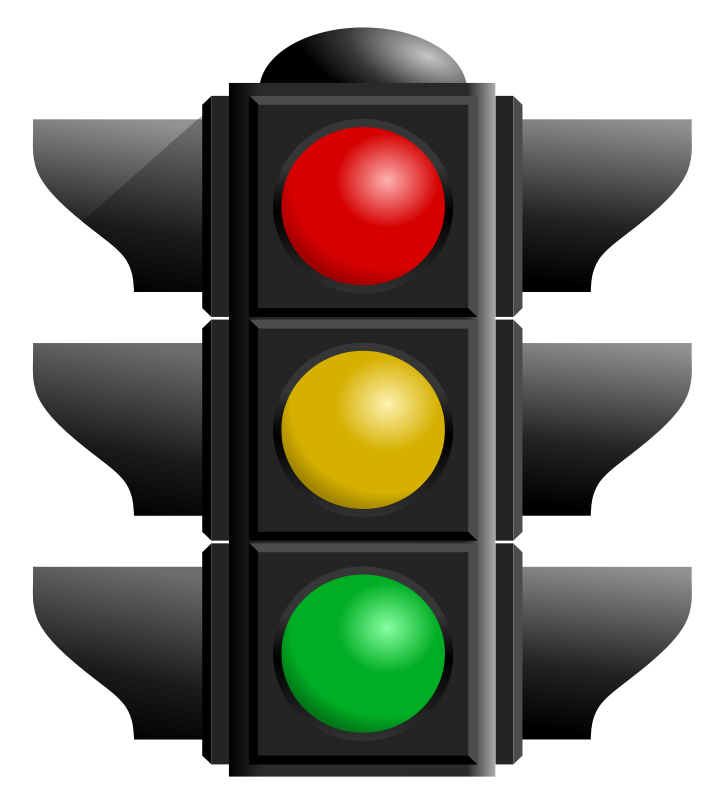
\includegraphics[width=1\textwidth]{images/traffic_light.png}
	\end{center}
	\end{column}

	\begin{column}{0.4\textwidth}
	\begin{center}
	\begin{tabular}{lll}
	\multicolumn{3}{l}{\textbf{Phase:}} \\
	green & : & 30 s \\
	yellow & : &  4 s \\
	red & : & 15 s \\
	yellow & : & 2 s \\
	green & : & 30 s\\
	\ \ \ \vdots&&\\
	\end{tabular}
	\end{center}
	\end{column}

	\begin{column}{0.3\textwidth}
	\begin{center}
	\begin{tabular}{l}
	\textbf{Green spans:} \\
	now: 42 s\\
	(51, 81) \\
	(102, 132) \\
	(153, 183) \\
	\ \ \ \ \vdots\\\\
	\end{tabular}
	\end{center}
	\end{column}
\end{columns}
\end{frame}

\begin{frame}{Calculate Velocity}
\[velocity = \frac{distance}{time}\]
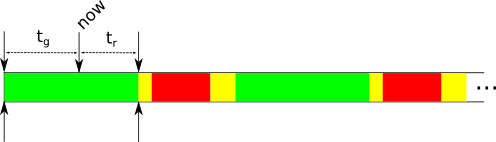
\includegraphics[width=1\textwidth]{images/algphases1.png}
\end{frame}

\begin{frame}{Calculate Velocity}
\[velocity = \frac{distance}{time}\]
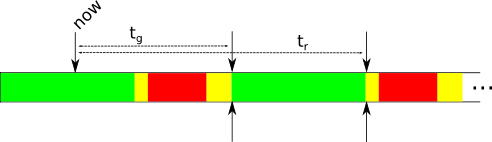
\includegraphics[width=1\textwidth]{images/algphases2.png}
\end{frame}

\begin{frame}{Calculate Velocity}
\[velocity = \frac{distance}{time}\]
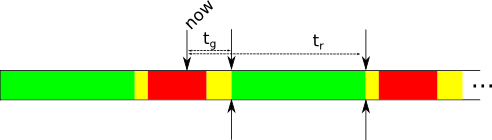
\includegraphics[width=1\textwidth]{images/algphases3.png}
\end{frame}






